% -----------------------------------------------
%   GeoTracking Block
% -----------------------------------------------
\subsection{The GeoTracking Block}
We enabled per-bundle tracking with the {\em GeoTracking} extension block, which collects both the logical hops that the bundle traverses and the bundle's trajectory through physical space. A {\em GeoTracking} block is a series of tracking entries prefaced by a small header containing parameters for maintaining the block and counting the entries.
\begin{figure}[!h]
\begin{center}
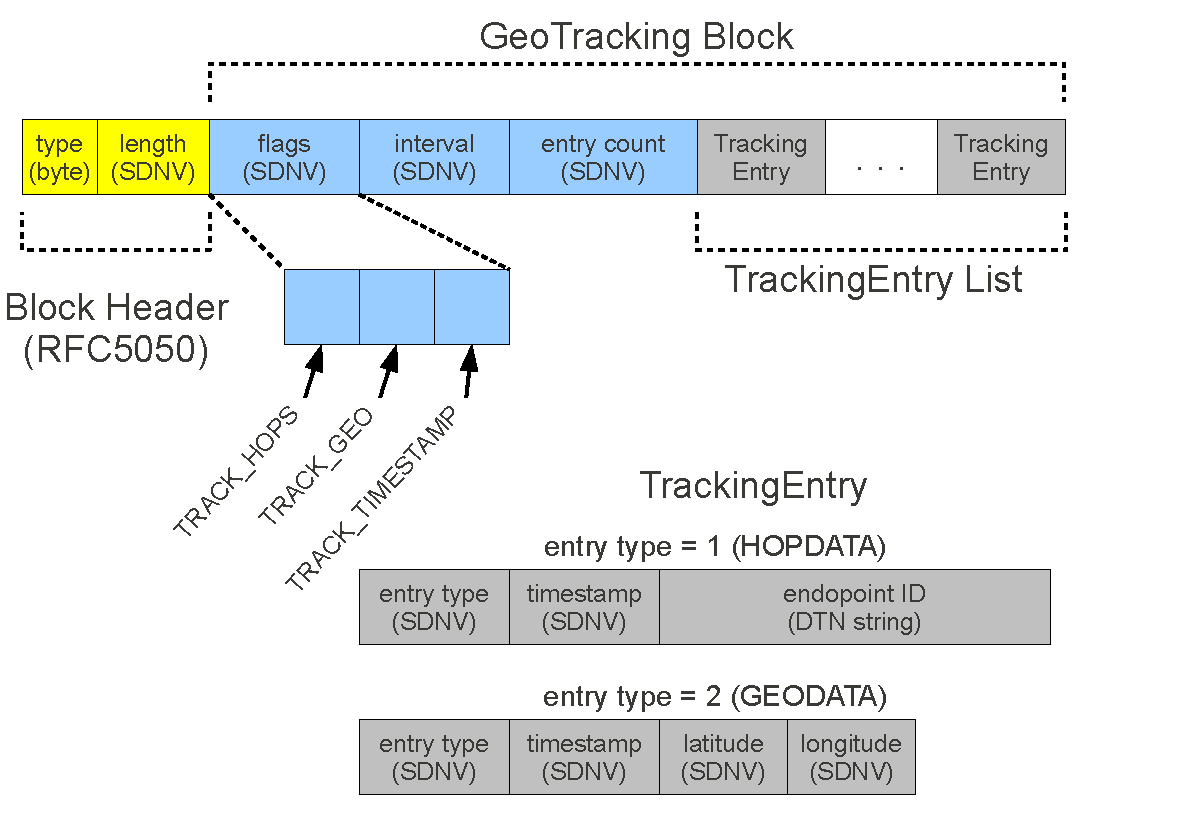
\includegraphics[width=.9\columnwidth]{figures/tracking-block.pdf}
\end{center}
\vspace{-.5cm}
\caption{Format of the GeoTracking Block}
\label{fig:tracking-block}
\vspace{-.25cm}
\end{figure}

\begin{sloppypar}
Figure~\ref{fig:tracking-block} depicts the {\em GeoTracking} block's format. The Block Header fields are specified by RFC5050\footnote{\scriptsize\url{http://tools.ietf.org/html/rfc5050}}. 
%In IBR-DTN, the block processor only deals with the contents of the block itself, and the Bundle Protocol Agent (BPA) strips off the block header. 
Each {\em GeoTracking} block contains three mandatory fields:
\begin{description*}
  \item[Flags.] The flags tell intermediate BPAs what information to append to the block. The flags are: {\bf TRACK\_HOPS} (0x01), {\bf TRACK\_GEO} (0x02), and {\bf TRACK\_TIMESTAMP} (0x04).
  \item[Interval.] The interval (in seconds) tells intermediate BPAs the frequency with which to append a new GEODATA tracking entry to the entry list.  
  \item[Entry Count.] The entry count keeps track of the number of tracking entries contained in the block.
\end{description*}
\end{sloppypar}

Keeping a {\em GeoTracking} block updated as the device storing the bundle moves is non-trivial for several reasons. First, there may be many bundles at a given node with {\em GeoTracking} blocks, and each bundle may have a different interval, requiring both responding to multiple timers and (in the case of IBR-DTN), reloading and storing each bundle from disk on every update. Instead, we maintain a global GPS log and update a bundle's associated {\em GeoTracking} block only when a bundle is serialized for sending. 
%Upon serialization, we examine the history of the GPS log and attach all of the appropriate entries to the {\em GeoTracking} block. 
To completely satisfy any arbitrary tracking interval requirement would require recording the node's location at an interval of the GCD of all of the tracking intervals, which may not be known {\em a priori}. We assume a host-specific agent that logs GPS data to a file at a fixed global interval; bundles can request a {\em less frequent} update. Each time a {\em GeoTracking} block is serialized, we scan the log file for the necessary entries and creates the necessary tracking entries for the {\em GeoTracking} block.

This approach still has some drawbacks.  First, it requires opening and reading a (potentially long) log file each time a {\em GeoTracking} block is serialized.  Second, in IBR-DTN, because there is no function to "finalize" the contents of a block prior to serializing, the GPS log must be parsed twice: once when the block processor calculates the block's length, and again when the actual serialization takes place.  
%In IBR-DTN both the {\bf getLength()} and {\bf serialize()} functions are {\bf const}, so it is not possible to modify any fields of the GeoTracking block itself to cache the state of the block when {\bf getLength()} is called.  
This technically creates a race condition between these two calls, where the GPS log may get longer between the two functions.  Resolving these issues completely may require some modifications to the serialization process of IBR-DTN and is reserved for future work.

%\subsubsection{GPS Coordinate Representation as SDNV} \label{gps-representation}
Our extension blocks represent GPS coordinates in signed degrees format, where latitude ranges from $-90^{\circ}$ to $90^{\circ}$ and longitude from $-180^{\circ}$ to $180^{\circ}$.  However, since the self-delimiting numeric values (SDNVs)\footnote{\scriptsize\url{http://tools.ietf.org/html/draft-irtf-dtnrg-sdnv-09}} used in the bundle protocol cannot represent floating point numbers or negative values, we make two transformations to encode the values in a {\em GeoTracking} block.  If $\theta<0$ we compute $\theta^{\prime}=\theta+360^{\circ}$.  Then we scale all coordinates up by a factor of $1048576$.  This gives us at least 20 bits of precision, which is more than enough for meter-level resolution.  When the blocks are received and deserialized, these transforms are simply reversed to get the floating point values.

We have implemented the {\em GeoTracking} block both in the core of IBR-DTN and within the Java API to support Java-based DTN applications.



